\documentclass[12pt, titlepage]{article}

\usepackage[pdftex]{graphicx}
\usepackage{booktabs}
\usepackage{tabularx}
\usepackage{hyperref}
\usepackage{float}
\hypersetup{
    colorlinks,
    citecolor=black,
    filecolor=black,
    linkcolor=red,
    urlcolor=blue
}
\usepackage[round]{natbib}

\title{SE 3XA3: Test Report\\Mari0}

\author{Team 9, Ninetendo
		\\ David Hobson - hobsondd
		\\ Jose Miguel Ballesteros - ballesjm
		\\ Jeff Pineda - pinedaj
}

\date{\today}

%% Comments

\usepackage{color}

\newif\ifcomments\commentstrue

\ifcomments
\newcommand{\authornote}[3]{\textcolor{#1}{[#3 ---#2]}}
\newcommand{\todo}[1]{\textcolor{red}{[TODO: #1]}}
\else
\newcommand{\authornote}[3]{}
\newcommand{\todo}[1]{}
\fi

\newcommand{\wss}[1]{\authornote{blue}{SS}{#1}}
\newcommand{\ds}[1]{\authornote{red}{DS}{#1}}
\newcommand{\mj}[1]{\authornote{red}{MSN}{#1}}
\newcommand{\cm}[1]{\authornote{red}{CM}{#1}}
\newcommand{\mh}[1]{\authornote{red}{MH}{#1}}

% team members should be added for each team, like the following
% all comments left by the TAs or the instructor should be addressed
% by a corresponding comment from the Team

\newcommand{\tm}[1]{\authornote{magenta}{Team}{#1}}


\begin{document}

\maketitle

\pagenumbering{roman}
\tableofcontents
\listoftables
\listoffigures

\newpage

\pagenumbering{arabic}

\section{Functional Requirements Evaluation}

\subsection{Input Testing}


\begin{figure}[h]
   \centering
   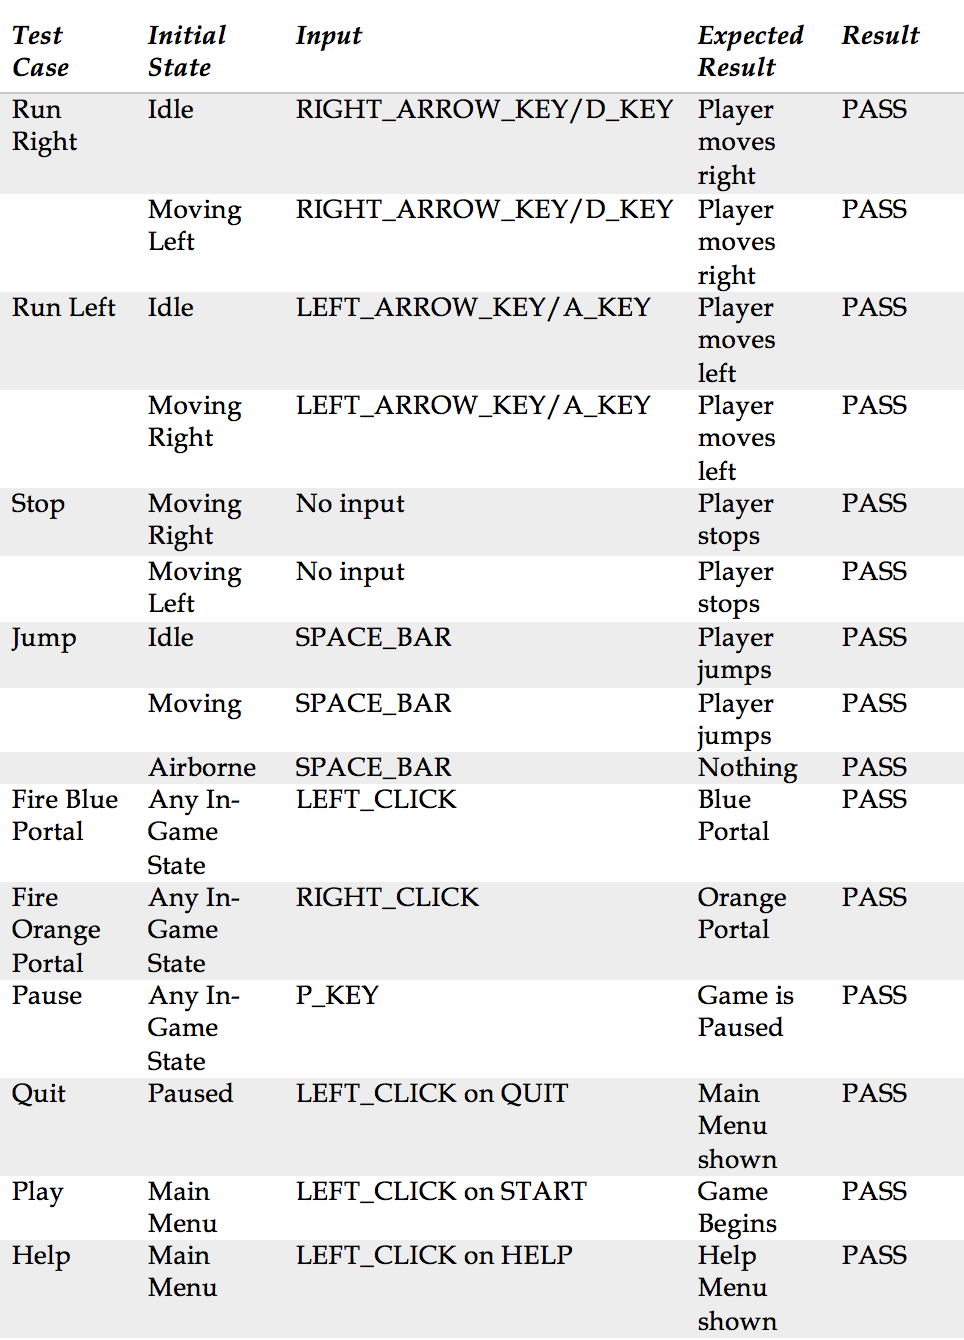
\includegraphics[scale=0.8]{Table1.png} % requires the graphicx package
   \label{fig:table1}
\end{figure}


\subsection{Collision Testing}

\begin{figure}[h]
   \centering
   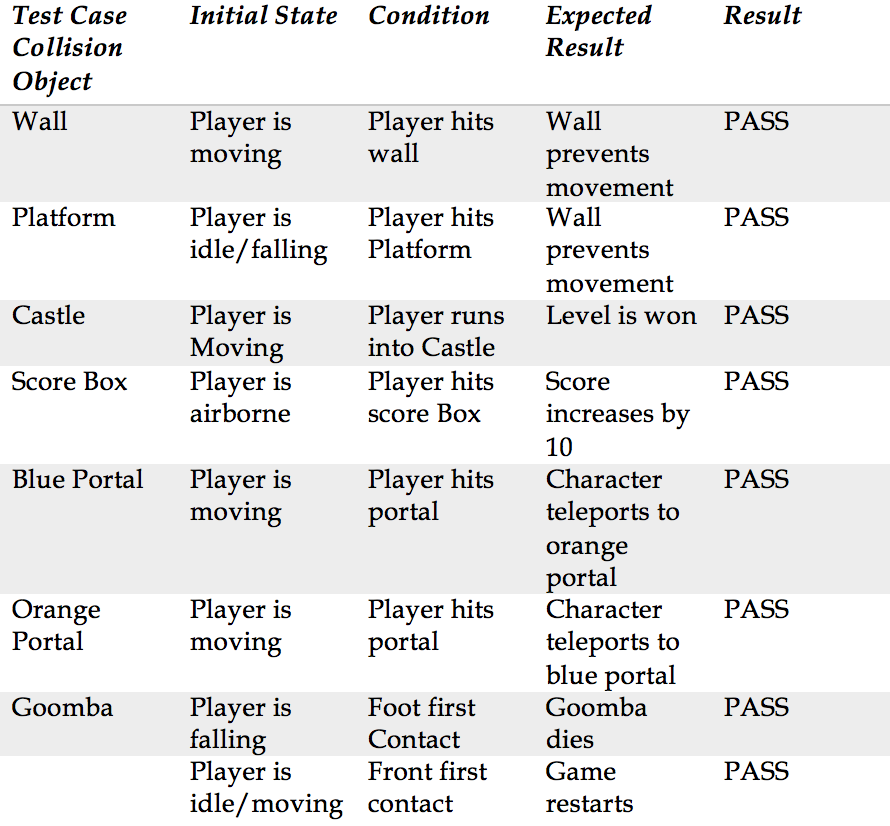
\includegraphics[scale=0.85]{Table2.png} % requires the graphicx package
   \label{fig:table2}
\end{figure}



\section{Nonfunctional Requirements Evaluation}

\textbf{Description:}
The following tests were executed by each member of our development team and a couple colleagues from our faculty. Engineering students were better suited for testing the current state of our project since it is an early development view of the open source game that is being recreated. Each participant was asked to give their honest feedback and suggestions.

\subsection{Look and Feel Requirements}

\begin{enumerate}

\item{Game Environment\\}

\textbf{Results: }All testers were able to explore all the game environments without issues.
					
\item{Game Hude/Interface\\}

\textbf{Results: }All testers stated that the location of the counter was not not obstructive in their opinion.

\end{enumerate}

\subsection{Usability and Humanity Requirements}

\begin{enumerate}

\item{Ease of Learning\\}

\textbf{Results: }All testers stated the game was easy to play and the controls were easy to learn.


\item{Entertainment\\}

\textbf{Results:} All testers stated that the game can be more enjoyable if it were stretched out to a longer period of time and had more gameplay, but is currently too short to provide a good amount of entertainment.

\end{enumerate}

\subsection{Performance Requirements}

\begin{enumerate}

\item{Controls/Commands\\}

\textbf{Results:} All testers noticed no delays or malfunction from the controls.

\end{enumerate}

\subsection{Operational and Environment Requirements}

\begin{enumerate}

\item{Operating System Support\\}

\textbf{Results:} Each tester was able to run the game on their own operating system. These include Windows and OSX 10.

\end{enumerate}

\subsection{Security Requirements}

\begin{enumerate}

\item{Altering Information\\}

\textbf{Results: }No tester indicated any type of alterations done to their current process or files.

\end{enumerate}


\subsection{Cultural Requirements}

\begin{enumerate}

\item{Spelling and Grammar\\}

\textbf{Results:} All testers indicated that the game had no spelling or grammar mistakes.

\item{Offensive Content\\}

\textbf{Results: }The testers indicated that they found no source of offensive content that would be directed at them or people from another culture.

\end{enumerate}

\subsection{Legal Requirements}

\begin{enumerate}

\item{License Adherence\\}

\textbf{Results: }The testers stated that they believe that the game is not breaching its current license.

\end{enumerate}

\subsection{Health and Safety Requirements}

\begin{enumerate}

\item{Epileptic Prevention\\}

\textbf{Results: }The testers indicated that they believe that the game would not trigger any epileptic seizures, although it is worth noting that non of the testers has ever had a history of epileptic seizures.

\end{enumerate}
	
\section{Comparison to Existing Implementation}	

This section will not be appropriate for every project.

\section{Unit Testing}

\section{Changes Due to Testing}
After the testing was complete no urgent fixes that interfered with the requirements were needed to be made.

\section{Automated Testing}
No automated testing methods were used for the testing of this product.
		
\section{Trace to Requirements}
		
\section{Trace to Modules}		

\section{Code Coverage Metrics}
No accurate code coverage metrics were achieved with our current test suit since it was all a result of manual and survey testing from other people. 

\bibliographystyle{plainnat}

\bibliography{SRS}

\end{document}